\chapter{
مفاهیم مقدماتی
}\label{S1}
\setcounter{page}{1}
\pagenumbering{arabic}

فصل اول پایان‌نامه به بیان تعاریف و مفاهیم اولیه اختصاص دارد.  معمولاً نمادگذاری و معرفی کلیدواژه‌های به کار رفته در پایان‌نامه در این فصل انجام می‌پذیرد و خواننده در صورت عدم آشنایی با مفهومی، می‌تواند به این فصل مراجعه نماید.

 توجه کنید که لزومی به اثبات همه مطالب و قضیه‌های مقدماتی، در این فصل، نیست و اصولاً چنین کاری شیوه مرسوم نیست. معمولاً انتخاب و ارجاع خواننده به یک کتاب معتبر یا هر مرجع معتبر دیگری بسیار مناسب‌تر است. چنین فصلی، جایی مناسب برای قضیه‌های «کلاسیک» درباره مساله مورد مطالعه است. توجه کنید که یک قضیه می‌تواند صورت‌های مختلفی داشته باشد و بهتر است از آن صورت مورد استفاده خود در این قسمت استفاده نمایید!

تعداد صفحات متوسط برای هر فصل بین 15 تا 25 صفحه و تعداد صفحات معمول برای پایان‌نامه بین 70 تا 100 صفحه است. 
به طور معمول پایان‌نامه‌های استاندارد دارای 4 یا 5 فصل هستند که در فصل اول مقدمات، در فصل‌های دوم و سوم مطالب نظری اصلی و در فصل چهارم برای رشته هایی نظیر آمار، آزمایش‌های عددی و تحلیل داده‌ها آورده می‌شود. فصل پنجم می‌تواند یک فصل کوتاه دو یا سه صفحه‌ای شامل جمع‌بندی، نتیجه‌گیری و پیشنهادات آینده باشد. 

برای زیرنویس معمولا از دستوری به این صورت\LTRfootnote{\lr{A footnote}} استفاده می‌شود. تعداد زیرنویس‌ها نبایستی خیلی زیاد باشد و بهتر است تنها به عنوان‌های تخصصی زیرنویس داد و مابقی واژگان را در بخش واژه‌نامه فارسی به انگلیسی  در انتهای پایان‌نامه آورد. فرمول‌های داخل متن به عنوان نمونه به صورت 
 $\{{Y_t}\}_{t=1}^T$
و فرمول‌های بین خط‌ها به عنوان نمونه به صورت زیر می‌آیند
\begin{equation}\label{graph_model}
\Pr(\mathbf{s},\mathbf{y})=\Pr(s_1)\Pr(y_1|s_1)\prod_{t=2}^{T}\Pr(s_t|s_1,\dots,s_{t-1})\Pr(y_t|y_1,\dots,y_{t-1},s_1,\dots,s_{t})
\end{equation}
و برای ارجاع دادن به این فرمول‌ از 
\eqref{graph_model} استفاده می‌شود. رعایت نیم‌فاصله‌ها در تمامی متن توصیه می‌شود. 
همچنین نقطه و کاما بایستی چسبیده به انتهای کلمه ماقبل و با فاصله از ابتدای کلمه بعد باشند. 

برای شروع یک پاراگراف جدید حتما بایستی یک خط فاصله خالی بین پاراگراف قبلی و بعدی بگذارید. برای آوردن شکل به صورت شکل 
\ref{fig.hmm}
عمل می‌کنیم. 
\begin{figure}[h!]
\centering
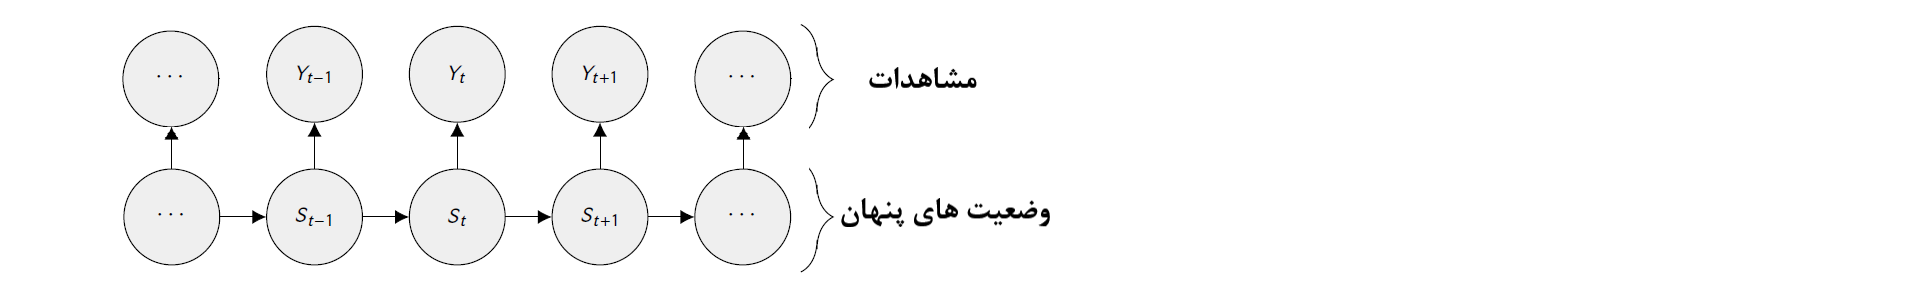
\includegraphics[scale=0.7]{HMM}
\caption{مصورسازی گرافی یک مدل مارکوف پنهان}
\label{fig.hmm}
\end{figure}

توجه کنید که اگر شکل را از منبعی به امانت گرفته‌اید بایستی حتما در زیرنویس شکل به آن منبع ارجاع دهید. 

برای ایجاد یک بخش جدید به صورت زیر عمل می‌کنیم. 

\section{بخش}

همینطور از نماد دو نقطه در فارسی تنها برای لیستی به صورت زیر استفاده می‌شود و قبل از فرمول‌ها استفاده از دونقطه توصیه نمی‌شود:
\begin{enumerate}
\item مورد اول
\item    مورد دوم ...
\end{enumerate}

برای ایجاد یک فرمول چند خطی می‌توانید به صورت زیر عمل کنید

\begin{align}
A &= B \nonumber \\ 
   & = C \label{alignformula}
\end{align}

برای ارجاع دادن به یک مرجع در متن به عنوان نمونه می‌توان به صورت 
 \cite{langrock2015b,pohle2017} عمل کرد.


\begin{defn}
عدد طبیعی 
$p$، 
$p\neq 1$، 
را اول گوییم، هرگاه به غیر از خودش و یک مقسوم علیه دیگری نداشته باشد.
\end{defn}


در این بخش یک شکل دیگر نیز برای نمونه می‌آوریم تا فهرست شکل‌ها کمی پربارتر باشد. 
\begin{figure}
\centering
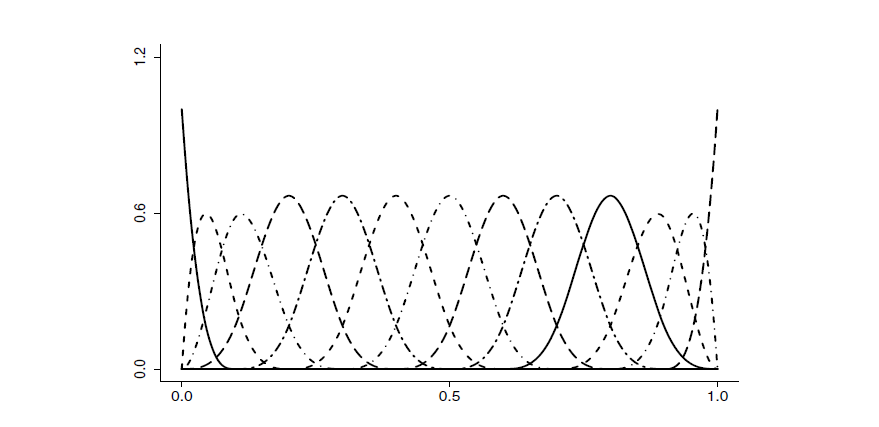
\includegraphics[scale=0.8]{spline}
\caption{پايه \lr{B}-اسپلاين درجه سه با استفاده از نه گره با فاصله‌هاي برابر در بازه $ (0,1) $}
\end{figure}

گاهی نیاز دارید تا یک شکل باکیفیت را در خود لاتک ایجاد کنید. نمونه‌ای از این کار در شکل 
\ref{spline-graph}
آورده شده است. توجه کنید که ارجاع به فرمول‌ها با پرانتز و ارجاع به شکل‌ها و جدول‌ها بدون پرانتز است. 

\begin{figure}
\centering
\begin{tikzpicture} [scale=2, thick]

\vertex[fill, scale = 2] (B11) at (2,2) [label=above:$B_{1,1}$] {};
\vertex[fill, scale = 2] (B21) at (2,1) [label=above:$B_{2,1}$] {};
\vertex[fill, scale = 2] (B31) at (2,0) [label=above:$B_{3,1}$] {};
\vertex[fill, scale = 2] (B41) at (2,-1) [label=above:$B_{4,1}$] {};
\vertex[fill, scale = 2] (B51) at (2,-2) [label=above:$B_{5,1}$] {};

\vertex[fill, scale = 2] (B12) at (3,1.5) [label=above:$B_{1,2}$] {};
\vertex[fill, scale = 2] (B22) at (3,0.5) [label=above:$B_{2,2}$] {};
\vertex[fill, scale = 2] (B32) at (3,-0.5) [label=above:$B_{3,2}$] {};
\vertex[fill, scale = 2] (B42) at (3,-1.5) [label=above:$B_{4,2}$] {};

\vertex[fill, scale = 2] (B13) at (4,1) [label=above:$B_{1,3}$] {};
\vertex[fill, scale = 2] (B23) at (4,0) [label=above:$B_{2,3}$] {};
\vertex[fill, scale = 2] (B33) at (4,-1) [label=above:$B_{3,3}$] {};

\vertex[fill, scale = 2] (B14) at (5,0.5) [label=above:$B_{1,4}$] {};
\vertex[fill, scale = 2] (B24) at (5,-0.5) [label=above:$B_{2,4}$] {};

\path
(B11) edge[-to] (B12)
(B21) edge[-to] (B12)
(B21) edge[-to] (B22)
(B31) edge[-to] (B22)
(B31) edge[-to] (B32)
(B41) edge[-to] (B32)
(B41) edge[-to] (B42)
(B51) edge[-to] (B42)
(B12) edge[-to] (B13)
(B22) edge[-to] (B13)
(B22) edge[-to] (B23)
(B32) edge[-to] (B23)
(B32) edge[-to] (B33)
(B42) edge[-to] (B33)
(B13) edge[-to] (B14)
(B23) edge[-to] (B14)
(B23) edge[-to] (B24)
(B33) edge[-to] (B24);
\end{tikzpicture}
\caption{نمايي از معادله بازگشتي تابع پايه \lr{B}-اسپلاين درجه 4}
\label{spline-graph}
\end{figure}


